%%%%%%%%%%%%%%%%%%%% author.tex %%%%%%%%%%%%%%%%%%%%%%%%%%%%%%%%%%%
%
% sample root file for your "contribution" to a contributed volume
%
% Use this file as a template for your own input.
%
%%%%%%%%%%%%%%%% Springer %%%%%%%%%%%%%%%%%%%%%%%%%%%%%%%%%%


% RECOMMENDED %%%%%%%%%%%%%%%%%%%%%%%%%%%%%%%%%%%%%%%%%%%%%%%%%%%
\documentclass[graybox]{styles/svmult}

% choose options for [] as required from the list
% in the Reference Guide

\usepackage[numbers]{natbib}
\usepackage{mathptmx}       % selects Times Roman as basic font
\usepackage{helvet}         % selects Helvetica as sans-serif font
\usepackage{courier}        % selects Courier as typewriter font
\usepackage{type1cm}        % activate if the above 3 fonts are
                            % not available on your system
%
\usepackage{makeidx}         % allows index generation
\usepackage{graphicx}        % standard LaTeX graphics tool
                             % when including figure files
\usepackage{multicol}        % used for the two-column index
\usepackage[bottom]{footmisc}% places footnotes at page bottom

% see the list of further useful packages
\newcommand{\blue}[1]{\textcolor{blue}{#1}} 		% proposed
\newcommand{\red}[1]{\textcolor{red}{#1}} 			% to be removed
\newcommand{\green}[1]{\textcolor{green}{#1}} 		% to be discussed?
\newcommand{\yellow}[1]{\textcolor{yellow}{#1}} 	% ????
\newcommand{\magenta}[1]{\textcolor{magenta}{#1}} 	% warning - requires

\newcommand{\ie}{\textit{i.e.,}\xspace}                   % i.e.,
\newcommand{\eg}{\textit{e.g.,}\xspace}                   % e.g.,
\newcommand{\etal}{\textit{et al.}\xspace}                % et al.
\newcommand{\facto}{\textit{, the facto,}\xspace}         %, the facto,
% in the Reference Guide

\makeindex             % used for the subject index
                       % please use the style svind.ist with
                       % your makeindex program

%%%%%%%%%%%%%%%%%%%%%%%%%%%%%%%%%%%%%%%%%%%%%%%%%%%%%%%%%%%%%%%%%%%%%%%%%%%%%%%%%%%%%%%%%

\begin{document}

\title*{On the Design of a Flexible Architecture for Virtualized Network Function Platforms}
% Use \titlerunning{Short Title} for an abbreviated version of
% your contribution title if the original one is too long
\author{Vin\'icius F. Garcia, Leonardo C. Marcuzzo, Giovanni V. Souza, Lucas Bondan, J\'eferson C. Nobre, Alberto E. Schaeffer-Filho, Carlos R. P. dos Santos, Lisandro Z. Granville, Elias P. Duarte Jr.}
% Use \authorrunning{Short Title} for an abbreviated version of
% your contribution title if the original one is too long
\institute{Vin\'icius F. Garcia, Leonardo C. Marcuzzo, Carlos R. P. dos Santos \at Federal University of Santa Maria, Santa Maria \email{\{vfulber,lmarcuzzo,csantos\}@inf.ufsm.br}
\and Giovanni V. Souza, Elias P. Duarte Jr. \at Federal University of Paran\'a, Curitiba \email{\{gvsouza,elias\}@inf.ufpr.br}
\and Lucas Bondan, Alberto E. Schaeffer-Filho, Lisandro Z. Granville \at Federal University of Rio Grande do Sul, Porto Alegre \email{\{lbondan,alberto,granville\}@inf.ufrgs.br}
\and J\'eferson C. Nobre \at University of Vale do Rio dos Sinos, Porto Alegre \email{jcnobre@unisinos.br}}
%
% Use the package "url.sty" to avoid
% problems with special characters
% used in your e-mail or web address
%
\maketitle

%\abstract*{
%The proper execution of Virtualized Network Functions (VNFs) depends on the employment of platforms specifically created to fulfill multiple NFV requirements (\textit{e.g.}, performance, integration, and management). However, existing VNF platforms implement different architectures, thus resulting in proprietary or limited solutions that do not always support important NFV specifications, such as VNF Components (VNFCs) and the Network Service Header (NSH). In this work, we introduce a comprehensive architecture for VNF platforms that supports the NFV requirements defined by the European Telecommunications Standards Institute (ETSI), while also enabling the execution of VNFCs and NSH. We implemented a VNF platform prototype, on which we conducted two different case studies, and report a series of performance evaluation experiments. Results demonstrate the intrinsic advantages of supporting VNFCs and NSH and show the flexibility of our architecture in distinct NFV scenarios.

%}

\abstract{
The proper execution of Virtualized Network Functions (VNFs) depends on the employment of platforms specifically created to fulfill multiple NFV requirements (\textit{e.g.}, performance, integration, and management). However, existing VNF platforms implement different architectures, thus resulting in proprietary or limited solutions that do not always support important NFV specifications, such as VNF Components (VNFCs) and the Network Service Header (NSH). In this work, we introduce a comprehensive architecture for VNF platforms that supports the NFV requirements defined by the European Telecommunications Standards Institute (ETSI), while also enabling the execution of VNFCs and NSH. We implemented a VNF platform prototype, on which we conducted two different case studies, and report a series of performance evaluation experiments. Results demonstrate the intrinsic advantages of supporting VNFCs and NSH and show the flexibility of our architecture in distinct NFV scenarios.

}


\section{Introduction}\label{INTRO}

Computer networks typically rely on dedicated equipment (\textit{i.e.}, middleboxes) to perform common network functions (\textit{e.g.}, NAT translation, intrusion detection and load balancing). However, despite the usual benefits of such middleboxes, including performance and reliability, they offer limited flexibility regarding the design and deployment of advanced network services. Network Functions Virtualization (NFV), in turn, is a networking paradigm that leverages virtualization technologies to decouple network functions from the physical equipment and run such functions as software that executes on commodity hardware~\cite{ETSI-2012}.

The adoption of NFV presents several benefits, including higher customization and the reduction of Capital and Operational Expenditures (CAPEX/OPEX). Multiple efforts are being conducted to foster the adoption of NFV technologies with the ultimate goal of encouraging the development of solid foundations that support advanced NFV solutions.

%New standards, models, and NFV enablers (systems used to support the execution of Virtual Network Functions - VNFs) are being developed by diverse organizations, such as the European Telecommunications Standards Institute (ETSI) and the Internet Engineering Task Force (IETF), as well as several working groups (\textit{e.g.}, ETSI NFV Industry Specification Groups - ISG, IRTF NFV Research Group - NFVRG, and IETF Service Function Chaining - SFC). The ultimate goal of these efforts is to encourage the development of solid foundations that support advanced NFV solutions.

Essentially, a VNF is divided into two main parts: the Network Function (NF) itself and the VNF platform.  NF corresponds to the software implementation responsible for packet processing, while the VNF platform is the environment that supports the execution of NFs. VNF platforms are designed taking into account the need to enable the creation of multiple network functions while consuming few computing resources. However, existing VNF platforms (\textit{e.g.}, ClickOS \cite{Martins-2014} and OpenNetVM \cite{Zhang-2016}) are not created using standardized architectures, thus resulting in solutions that are either proprietary or present serious limitations, such as the lack of support for advanced NFV specifications, in particular Network Service Header (NSH) -- a packet header that enables the creation of dynamic service planes \cite{Quinn-2018}.

%in particular VNF Components (VNFCs) \cite{ISG-2013} -- individual elements consisting of some or all of the VNF functionality -- and Network Service Header (NSH) -- a packet header that enables the creation of dynamic service planes \cite{Quinn-2018}.

%In this paper, we introduce a comprehensive architecture for VNF platforms that strictly adheres to ETSI requirements and provides support for VNFCs and NSH. Our key contributions are: i) the design of the core elements of a flexible architecture for VNF platforms that support VNFCs and NSH; ii) the development of a VNF platform prototype based on the proposed reference architecture; and iii) the identification of critical features provided by both VNFCs and NSH that enable the development of advanced network services.

In this paper, we introduce a comprehensive architecture for VNF platforms that strictly adheres to ETSI requirements and provides support for NSH. Our key contributions are: i) the development of a VNF platform prototype based on ETSI requirements; and ii) the identification of critical features provided by NSH that enables the development of advanced network services.

The remaining of this paper is organized as follows. Section II presents the background on NFV along with its main components, basic requirements, and a review of the literature. In Section III, we propose a architecture for developing VNFs with support for NSH, and instantiate this architecture by describing a running prototype platform implemented to support virtualized network functions. In Section IV, we evaluate the performance of our prototype. Finally, in Section V, we conclude this paper with final remarks and an outline of future work.

\section{Background and Related Work} \label{BACK}

In this section, we present the background on Network Functions Virtualization (NFV) and Virtualized Network Function (VNF). We also discuss the characteristics and limitations of existing VNF platforms.

\subsection{Network Function Virtualization in a Nutshell} \label{VISAO}

NFV aims to implement Network Functions (NFs) in software, so they can run on commodity hardware by employing common virtualization technologies \cite{ETSI-2012}. Two of the most relevant standardization bodies are expending considerable energy in defining models, methodologies, and concepts in this area: the European Telecommunications Standards Institute (ETSI) and the Internet Engineering Task Force (IETF).

The NFV architectural framework \cite{GS-2014} defined by ETSI is composed of three functional blocks: NFV Infrastructure (NFVI), NFV Management and Orchestration (NFV MANO), and Virtualized Network Functions (VNF). NFVI is the collection of physical resources (\textit{e.g.}, processing, storage, and network) needed to execute VNFs. NFV MANO in turn encompasses: the Virtualized Infrastructure Manager (VIM), which controls the physical/software infrastructure; the VNF Manager (VNFM), which is responsible for VNF lifecycle operations (\textit{e.g.}, instantiation, termination, scaling, and migrations); and the NFV Orchestrator (NFVO), which enables the management of network services. Finally, the VNF functional block itself represents the network functions that run on VNF platforms.

Because of the development flexibility offered by NFV, advanced network services can be quickly created and deployed, such as NFV-based security solutions (\textit{e.g.}, DeMONS \cite{Garcia-2018}, VFence \cite{Jakaria-2016}, and \cite{Cunha-2018}), \blue{as well as common network services, such as DHCP, DNS and Routing}.

%These sophisticated functions are designed through the composition of multiple VNF Components (VNFC) \cite{GS-2014-2}. Usually, a standalone VNFC performs a specific functionality with lower complexity, but the combination of VNFCs enables the creation of complete VNFs. In general, a VNFC is also a virtualized element, but its lifecycle depends on its parent VNF.

The IETF has been working on standardizing the Service Function Chain (SFC) \cite{Joel-2015}, which consists of multiple VNFs working together in a composition that provides a network service. In addition to internal VNFs, a SFC also includes boundary nodes (\textit{i.e.},  incoming and outgoing points of traffic) and steering specifications. One way to implement those SFCs is by using the architecture defined in the IETF's Request for Comments (RFC) number 7665 \cite{Joel-2015}. In that RFC, a Network Service Header (NSH) \cite{Quinn-2018} is employed to enable packets to traverse a specific path of VNFs. Each VNF, in turn, can either be NSH-aware or not. NSH-aware VNFs make a request to a proxy element to remove the NSH before processing, after which the proxy element is again invoked to update/reinsert the NSH element. Alternatively, VNFs can process NSH themselves, without relying on external elements.

An NSH encapsulates L3 packets as they are processed by the SFC, and carries information about the Service Function Path (SFP), the current packet location in the SFP, and meta-data provided by the VNFs during packet processing.  NSH is subdivided into three meta-headers: Base Header, Service Path Header, and Context Header. The Base Header provides general information about the protocol itself and the next meta-headers data. This meta-header (4 bytes), in turn, carries 5 fields (\textit{i.e.}, version, O bit, TTL, length, and meta-data type), in addition to reserved space for future protocol use. The Service Path Header is also formed by 4 bytes and has 2 fields: Service Path Identifier (identifies the SFC's SFP) and the Service Index (provides the location of the packet in the SFP). Finally, the Context Header can be fixed (16 bytes) or variable to carry meta-data information as the SFC is processed.

%VNF platforms are specially designed to host VNFs and their associated components. The ETSI lists the basic requirements for developing such platforms (\textit{e.g.}, hardware independence, elasticity, reliability) \cite{SWA-2014}. The ETSI also specifies that a VNF platform must host VNFs independently of the underlying hardware. Furthermore, VNF platforms must provide the flexibility expected from the NFV paradigm to support the operations of deployment, scaling, and migration.

VNF platforms are specially designed to host VNFs and their associated components. The ETSI lists the basic requirements for developing such platforms (\textit{e.g.}, hardware independence, elasticity, reliability) \cite{SWA-2014}. The ETSI also specifies that a VNF platform must host VNFs independently of the underlying hardware. Furthermore, VNF platforms must provide the flexibility expected from the NFV paradigm to support the operations of deployment, scaling, and migration.

%The fundamental NFV requirements that must  be fulfilled by VNF platforms in order to support VNF execution, according to the ETSI \cite{ISG-2013}, are:

%\begin{itemize}
%    \item \textbf{Portability} -- VNFs from different vendors should execute independently of platforms and infrastructures employed. Therefore, it is essential to use unified interfaces that isolate the instances of VNFs from the associated physical infrastructure.

%    \item \textbf{Performance} -- The use of NFV-based technologies may lead to performance degradation in comparison with the performance of middleboxes. That happens mostly due to non-optimized network hardware and inadequate software solutions (\textit {i.e.}, without virtualization optimizations).

%    \item \textbf{Integration} -- Network operators must be able to employ multiple physical servers, hypervisors, and VNFs of different technologies without limitations.

%    \item \textbf{Management and Orchestration} -- VNFs should provide adequate management interfaces for both network operators and other functional blocks of the NFV architecture. Examples of Management and Orchestration requirements include easy and efficient VNF configuration, instantiation, provisioning, and design \cite{Bondan-2014}.

%    \item \textbf{Scalability} -- VNFs must be easily scaled, instantiated, and migrated to support the ever-changing needs of network operators.
%\end{itemize}

%Several aspects of VNF platforms, however, are still unexplored in the literature. For example, the lack of standards for the internal modules have led to several solutions, mostly created without integration in mind neither support for well-accepted management models. Existing platforms, detailed next, usually support only a single programming language, run on very specific hypervisors, do not describe a formal architecture, and do not fulfill all the above requirements defined by the ETSI.

Several aspects of VNF platforms, however, are still unexplored in the literature. For example, the lack of standardization on existing VNFs platforms, mostly created without a well defined architecture and missing features such as NSH and SFC support. Existing platforms, detailed next, usually support only a single programming language, run on very specific hypervisors, do not describe a formal architecture, and do not fulfill all the above requirements defined by the ETSI.


\subsection{VNF Platforms} \label{PEVNFS}

Many research efforts concentrate on creating VNF platforms that are capable of executing NFs. However, these VNF platforms do not provide support for more recent NFV specifications, such as NSH. Still, two of the most important VNF platforms today are ClickOS and OpenNetVM, described next.

ClickOS \cite{Martins-2014} is an optimized platform for running NFs based on Mini-OS, \textit{netmap}, and \textit{Click Modular Router}. ClickOS uses paravirtualization techniques along with several modifications in both Xen and VALE to support fast packet I/O, being able to saturate 10GbE links with a single processing core. Alas, the ClickOS architecture is monolithic and inflexible and supports only a single packet acceleration tool for sending and receiving network traffic to an indivisible NF.

OpenNetVM \cite{Zhang-2016} is a simplified platform that uses containers to execute VNFs on commodity servers along with the packet acceleration framework DPDK \cite{Intel-2014}. OpenNetVM meets the ETSI scalability requirements because of its lower overhead due to the use of containers, which are a lightweight solution in comparison with virtual machines. The OpenNetVM architecture consists of a packet acceleration tool interconnecting VNFs with Virtualized NICs (VNICs). NFs are created as a single component within a proprietary framework and are deployed on a container core. OpenNetVM also provides an internal router implemented using shared memory, which steers network traffic between multiple VNFs.

Both ClickOS and OpenNetVM unfortunately lack support for important VNF elements (\textit{e.g.}, VNFCs and NSH). The ClickOS architecture is straightforward and does not have any native management method, providing only a minimalist environment to execute simple NFs. Despite OpenNetVM's internal traffic router, the platform is restricted to a single packet acceleration tool and a single packet processing framework, both deployed on a container core and managed by an external native agent. Furthermore, these platforms do not meet all of the requirements specified by the ETSI. ClickOS, for example, can only be executed on the Xen hypervisor and every control operation is performed locally through the XenStore. Also, OpenNetVM presents limitations related to NF instantiation (due to hardware device sharing), portability (migrations are only possible between compatible infrastructures), and security issues with containers (single kernel sharing) \cite{Manco-2017}.

\section{VNF Platform Architecture and Prototype} \label{ARCH}

In this section, we introduce an architecture for VNF platforms which supports SFC chaining using NSH. The proposed architecture is designed to be flexible and technology agnostic. Ultimately, we expect this architecture to serve as a template for designing new systems and re-engineering existing ones.

\subsection{Architecture Overview}

Currently, there is no \textit{de facto} standard for the design and development of VNF platforms, from neither industry nor academia. VNF platforms, however, must be developed to meet multiple strict requirements (\textit{e.g.}, portability, performance, integration, management, and scalability), in order to fulfill the needs of modern networks. Furthermore, the NFV area is evolving, with new technologies being created continuously. Therefore, it is essential to design flexible solutions that support new NFV Enablers (\textit{i.e.}, existing frameworks and technologies that contribute to the development and implementation of NFV) from an ever increasing number of players in the NFV market. VNF platforms must also be created with integration in mind. There are several systems (OSS/BSS, Hypervisors) and elements (NFVI, VNFM, EMS) that must work together with multiple VNFs in order to adequately provide virtualized network services \cite{GS-2014}. % Furthermore, each running VNF can also be decomposed into multiple VNF Components (VNFCs), each performing some specific operation but acting in consonance with others to process network traffic.

% \red{Talvez tirar o nome dos modulos? Reduzido para ficar mais parecido com módulos do coov, sem IR e extended agents? Figura?}

\begin{figure}[!ht]
    \centering
    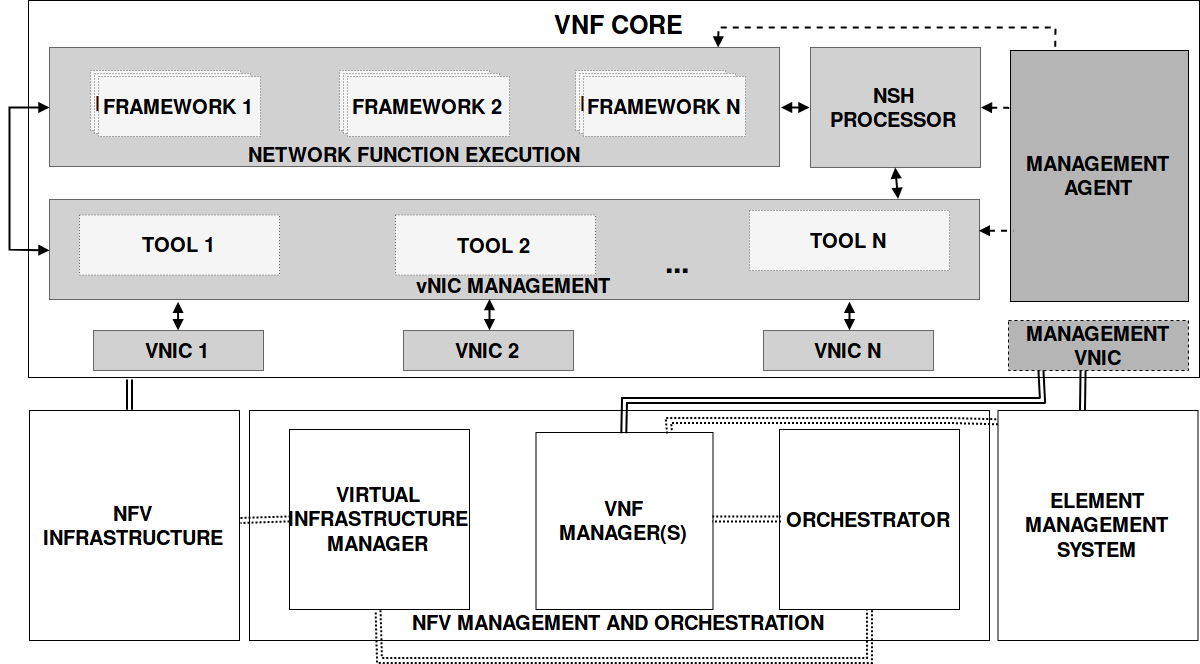
\includegraphics[width=\textwidth]{images/FullArchitecture_MOD.png}
    \caption{\label{vnfGeneric} VNF Platform Architecture}
\end{figure}

In this context, we propose a generic and flexible architecture for VNF platforms, (Figure~\ref{vnfGeneric}). The proposed platform consists of multiple modules, deployed on a host operating system (called here VNF Core): an module responsible for management access of Virtual Network Interfaces (vNIC), being the main point of input/output of packets from the architecture, a module consisting of a framework for development and execution of network functions, a management agent responsible for configuration of the host operating system and the other modules and, finally, a NSH Processor which provides an abstraction for the network functions regarding the existence of NSH packets.

% \blue{Packets I/O when executed by the native network stack in traditional operating systems, is not optimized to support the performance requirements of high-speed networks (\textit{e.g.}, 40GbE/100GbE). To tackle this problem, packet acceleration tools (\textit{e.g.}, Intel DPDK \cite{Intel-2014}, NetMap \cite{Rizzo-2012}) have been proposed and extensively evaluated. Once the network packets enter the VNF, they are forwarded internally through communication channels (\textit{e.g.}, using shared memory, pipes, sockets) to the NSH Processor if the VNF is in a service chain, otherwise being forwarded directly to the Network Functions.}

\blue{The IETF specified the Network Service Header (NSH) that is inserted in packets/frames to provide service function paths \cite{Quinn-2018}. However, despite its advantages, the use of NSH is optional to steer traffic across multiple VNFs. In order to support both cases, we define the NSH Processor, which acts on the specific NSH fields that may be modified when traversing a network path (\textit{i.e.,} the Service Index - SI; and Context Header - CH). NSHP provides the following operations: NSH removal, NSH reinsertion, CH retrieval, and CH update.}

Packets are then received by the development frameworks used to implement network functions. Basically, these frameworks include applications (\textit{e.g.}, Click Modular Router \cite{Kohler-2000} and Vector Packet Processing \cite{Cisco-2018}), programming languages (\textit{e.g.}, C, C++, Python), libraries (\textit{e.g.}, Scapy, libtins, libnet), or even single routines that support the construction and handling of network packets.

\blue{All the described modules are controlled by an management agent, which is responsible for to monitoring and controling the execution of VNFs. Once a VNF is executing, retrieve operations can be used to gather information about the VNF instance (\textit{e.g.}, VNF ID, network interfaces), measuring performance indicators from the VNF Core (\textit{e.g.}, CPU, memory, and network usage) and providing information retrieved from the extended agents deployed in the VNF platform.}

% upon receiving a configuration file, does the validation, extracts the relevant information for deploying the VNF, and

%The module is controlled by the Management Agent and is used to monitor/control each network function or component. It is supposed to be developed by the creator of the VNF/VNFC, as it acts on the individual management data of those implementations (\textit{e.g.}, number of discarded packets by a firewall). This module must provide at least one standard operation which we call ``list''. This operation is used by MA to discover all the management data that can be accessed by network operators.

%All the described modules are controlled by the MA, which upon receiving a VNFP (MA-MV interface), does the validation, extracts the relevant information for deploying the VNF, and configures the internal modules accordingly.


%For example, VNFP may contain information regarding the set of VNFCs that compose a VNF, which is essential for the Internal Router to forward the traffic to the proper components. The initial request for VNF deployment must also provide more specific information, such as the extended agents to be instantiated together with the network functions.

%The Management Agent is also responsible for extracting the implementation source code of the VNFCs from the VNFP, request the Packet Processing Subsystem to create the associated communication channels, and to start the execution of VNFCs (Figure \ref{vnfGeneric} MA-EA and PPSF-EA). Once this operation concludes, PPS returns a success/failure confirmation to the Management Agent (MA-PPS). In case of failures, rollback mechanisms may be employed to abort the instantiation process properly. When NSH is used, the Management Agent starts the NSH Processor (MA-NSHP). NSHP then creates a communication channel with the Packet Processing Subsystem (NSHP-PPS) to allow the network functions to access the NSH context header. VNICs are connected to the Virtual Network Subsystem (VNS-VNIC) based on the original request specified in the VNFP, processed by the MA (MA-VNS). The overall configuration of the VNF Platform is depicted in Figure \ref{FIG:CONF}.

%Finally, the Internal Router is initiated with two default communication channels: IR-VNS and IR-PPS. The former is used by the IR to retrieve network packets from the VNS, while the latter is used by VNFCs to access the packets to be processed. A third connection labeled IR-NSHP is used (i) to remove the NSH before any VNFC and (ii) to reinsert the NSH after the last VNFC of the path.

% \blue{The architecture described in this section defines modules responsible for the deployment of VNFs with SFC support\cite{Joel-2015}. We believe the architecture can provide a valuable reference for the design and development of VNF platforms, working as a guideline to integrate distinct modules in order to create complete solutions.}

\subsection{Prototype Development}\label{PROTO}

% Raniery (06/08): no geral a seção pode ser condensada em um texto mais limpo e direto. Por exemplo, a maior parte das explicações na segunda subseção já é mencionada antes. Na mesma linha, fiquei com a sensação de que alguns elements já são apresentados e discutidos na seção anterior. ACHO que toda a segunda subseção pode ser removida. Talvez algumas poucas partes possam migrar para outros lugares

%VINÍCIUS: Sim de fato, algumas coisas estão um pouco repetidas, porém aqui nos damos nomes aos bois, a idéia é justamente dizer, olha para tais e tais módulos, usamos tais e tais ténologias. Vou trabalhar com a idéia de não passar dados de relações e etc, mas de fato identificar detalhes de implementação.

% Raniery (06/08): Fiquei na dúvida se as informações estão consistentes ao longo da seção. Por exemplo fala sobre shared memory, L2 socket, L3 socket, system call.

%VINÍCIUS: Sim tudo é usado mesmo
%Shared Memory: comunicação entre os módulos internos a plataforma.
%L2 Socket: ferramenta de rede virtual para acessar as VNICs.
%L3 Scoket: Comunicação entre o PPS e os frameworks.
%System Call: Método de instanciação dos frameworks de processamento de pacotes

As a proof of concept of the proposed architecture presented in the previous section, we implemented a prototype that consists of a VNF platform that employs modern and well-accepted NFV enablers. In this context a NFV enabler is any technology used as a basis for the development of NFV ecosystems \cite{ETSI-2012}, such as hypervisors, packet acceleration frameworks, virtual routers, and operating systems.

\subsection{NFV enablers}

In our solution, we employ the following technologies:

% In this section we present a prototype based on the architecture previously defined in section \ref{ARCH}. The prototype was built on top of a Debian operating system (acting as VNF Core), while the internal modules were developed using modern NFV Enablers.
% In this section, a prototype based on the architecture previously defined in section \ref{ARCH} is presented. The prototype was built on top of a Debian operating system, with some components being specifically developed for the platform and others based on readily available frameworks. First, those frameworks (\textit{i.e.,} NFV Enablers), as well as the reasons of using they are briefly introduced. Then, the development process of the remaining components and how they interact with the enablers is presented. Finally, the interaction between those components inside the platform and with the NFV ecosystem is discussed.
% \subsection{NFV Enablers}
% An "NFV Enabler" is any technology that can be used as basis for the development of NFV ecosystems \cite{NFVPaper}, for example, hypervisors, packet acceleration frameworks, virtual routers, and operating systems. In the context of this paper, we have chosen the following technologies as basis for developed prototype, which aims to enable us in the analysis of the architectural design we presented previously. %, and analyze the NFV requirements and proposed modules of the   % For the platform development, some modules have functions that can be performed by already available frameworks, and due to the flexibility of the platform, they could be used to perform these functions, although this does not limits the usage of custom modules developed for the VNF.

\begin{itemize}
    \item \textbf{Click Modular Router} -- a well-known packet processing framework that provides an extensive list of network elements, native support for packet acceleration frameworks, and built-in control methods. The Click framework has been extensively investigated in academia and employed in several efforts to develop VNF platforms, such as ClickOS \cite{Martins-2014}, Click-on-OSv \cite{Marcuzzo-2018}, and the platform proposed by Bu \textit{et al.} \cite{Bu-2018}; % Click is used in our solution as the framework for packet processing (Python 3 is also supported), since its built-in elements enable the development of heterogeneous network functions and can be extended to support novel networking protocols.

      % \item \textbf{Click Modular Router}: the Click Modular Router is a well-known packet processing framework with an extensive list of network elements, native support for packet acceleration technologies, and built-in management methods. This framework was used in several efforts to develop VNF platforms, such as in \cite{clickos} and \cite{Bu-2018}. In the platform, it is used as the default packet processing framework, since its built-in elements make network function development easy for users (without having to implement the entire packet processing) and can also be extended to support new elements.

      \item \textbf{Intel Data Plane Development Kit (DPDK)} -- a packet acceleration framework that provides high throughput with reduced resource consumption (by using PCI passthrough and zero-copy) and supports multiple network interface cards (including paravirtualized ones, such as \texttt{virtio} and \texttt{netfront}); % DPDK was employed because it is one of the most widely accepted solutions today.

      % \item \textbf{Data Plane Development Kit}: the Intel Data Plane Development Kit (DPDK) is a packet acceleration framework, which is used as the default Virtual Network Subsystem, being capable of high performance with reduced resource usage, support for multiple different network interface cards (including paravirtualized ones such as virtio and netfront), as well as technologies such as polling, PCI passthrough and zero copy.

      \item \textbf{RESTful Web Services} -- an architectural style for the provisioning of Web Services (WSs) with simplified access to resources \cite{Roman-2005}. RESTful web services are lighter than traditional SOAP-based WSs and are used here as the basis for the management agent to export performance statistics regarding the VNF platform, and to receive management requests from an external VNFM or EMS.

    % \item \textbf{RESTful Web Services}: an implementation of a REST Web Server is used for management and collection of statistics of the VNF platform. By using an Web API, the platform can be externally managed thorugh a dedicated management interface, detaching its management from the network where it is used to process packets.
\end{itemize}

Furthermore, we have chosen Debian as the operating system for the VNF Core. Although this operating system is not explicitly designed to support the NFV requirements (\textit{e.g.}, performance), this decision enabled us to focus on the development of the internal modules without concerns about software compatibility, thus enabling the analysis of the architecture from the functional point-of-view. However, the development of NFV platforms for production environments should benefit from more recent solutions such as  OSv, CoreOS, MiniOS, and Alpine.

% [ref1]: http://citeseerx.ist.psu.edu/viewdoc/download?doi=10.1.1.671.8671&rep=rep1&type=pdf

%\begin{figure*}[ht]
%\centering
%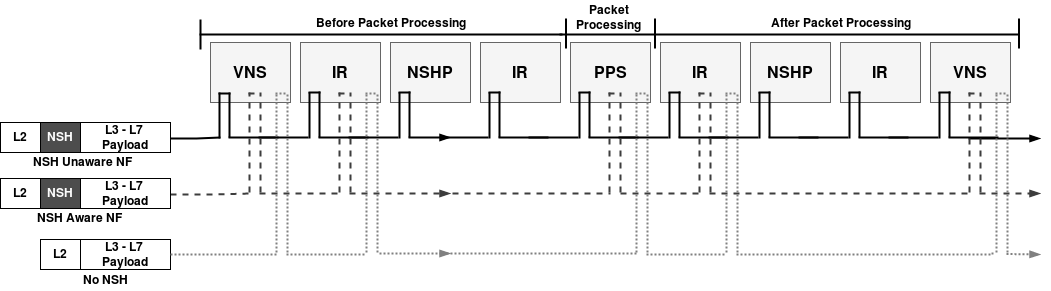
\includegraphics[width=.8\textwidth]{images/PlatformFlow.png}
%\caption{Prototype Platform Execution Scenarios}
%\label{FIG:PLATEXEC}
%\end{figure*}

\subsection{Platform Prototype}

% The platform was built on top of a minimal image of the operating system Debian 9. Packages were installed specifically to built an environment to provide the main functionalities of VNF systems introduced in the previous section. There are two main process in the platform: the data plane process and the management plane process. The VNFs platform architecture modules are implemented as sub-process, being the data plane process parent of the VNS, IR, NSHP, and PPS and the management plane process parent of the MA and EA.

For handling the vNICs, we initially chose DPDK. However, the platform also supports L2 Sockets to provide increased flexibility. These two options are available and can be selected according to the specific needs of the operator\footnote{The polling method of DPDK is inefficient regarding to CPU resources, while L2 Sockets are not able to achieve high throughput.}. Although we have employed these two solutions, other solutions (\textit{e.g.}, PF\_RING, and netmap) could be used without significant implementation efforts.

% The Virtual Network Subsystem is provided by two tools: the DPDK and L2 sockets. These tools are used to receive network packets from the virtualized interfaces and forward them to the internal router. Although only the DPDK and L2 sockets were made available in the platform, any framework compatible with Linux and with paravirtualized network drivers, such as netmap and PF\_RING, could be inserted in the platform and provided for the VNFs developers with minimum programming efforts.
%VINICIUS: fiz alterações aqui, o Internal Router não tem duas opções de comunicação, mas sim, um tipo para módulos internos e outro para os módulos externos, aqui a escrita passou a ideia errada do que realmente acontece na implementação.

%The Internal Router communicates with other internal modules of the architecture (\textit{i.e.}, Virtual Network Subsystem and NSH Processor) on shared-memory to guarantee high performance. For the communication with PPS (\textit{i.e.} NFs or VNFCs), L3 Sockets are employed, which may affect the latency and throughput when compared to shared memory. However, L3 Sockets provide greater flexibility in the development of NFs and VNFCs.

%platform independence during the NF (or VNFCs) development and a higher compatibility with current NFs implementations.}

%The Internal Router can communicate with other internal modules of the architecture (e.g., NSHP and MA) by using shared memory or conventional L3 Sockets. The prior provides greater performance, however doesn't allow the internal modules to be decoupled from the VNF platform (i.e., be executed outside the user space), while the later may affect latency. Shared memory is also used for communication between multiple VNFCs, while sockets are used by the NFs to receive/send network packets from/to the IR.

% forward packets to the individual VNFCs by using shared memory or conventional L3 Sockets. The prior provides greater performance, however doesn't allow the internal modules to be decoupled from the VNF platform (i.e., be executed outside the user space), while the later may affect latency. Shared memory is also used for  inter-related process communication between the IR and the Management Agent.
% The Internal Router is responsible for forwarding packets to the other VNF platform modules, ensuring they arrive at the correct destination. As such, it can forward packets by using shared memory areas (preferred due to its performance, however requires modifications on external modules) or by using sockets, achieving greater compatibility but typically with an extra delay. The prototype internal data plane modules are implemented supporting inter-process memory sharing which is used to perform the communication. In the other hand, the NFs deployed in the platform communicates the Internal Router through generic L3 sockets, being platform agnostic (\textit{i.e.}, the functions can be used in other platforms without any modification).

The NSH Processor operates as a proxy during the platform execution and can be enabled by the network operator. When enabled, packets first pass through the NSHP in order to remove NSH before steering the packets to the network function (\textit{i.e.}, CMR or Python-based NFs/VNFCs), and for NSH reinsertion before forwarding processed packets back to the vNIC (\textit{i.e.}, DPDK or L2 Sockets). The NFs, when necessary, can access the NSH Context Header to retrieve or replace content using specific libraries we developed (both in Python and CMR)\footnote{By the time of writing, we opted to support only Context Headers of fixed-length \cite{Quinn-2018}.}. Notice that, during the NSHP reinsertion operation, the Service Index field is updated.

%the NSHP removes the NSH specific header from each network packet prior delivering them to Packet Processing Subsystem (i.e., the NFs), and reinserts it before sending to the Virtual Network Subsystem (i.e., DPDK or L2 Socket). The NFs, when necessary, can access the NSH's Context Header to retrieve or replace its content by using specific functions (both in Python and CMR) we developed to enable these operations. \footnote{By the time of this work, we opted to support only Context Headers of fixed-lenght \cite{rfc8300}}. It's important to notice that, prior reinserting the NSH, the Service Index field is updated by the NSHP.

% Finally, after the packets are processed by the PPS, the Service Index field is updated and the data is encapsulated back to the NSH.

%As for the NSH Processor, it was developed as an optional activation element in the platform prototype. The NSH Processor acts like a proxy during the platform execution. When this module is active, before the packets be steered for the Packet Processing Subsystem, they are processed in order to remove and keep the NSH. Every processed packet is marked in order to identify it during the NSH reinsertion process. The NFs, when necessary, can request the NSH's Context Header retrieving or replacement through an standard REST interface provided by the NSHP. The prototype NSH Processor module works with fixed-length Context Headers \cite{rfc8300}. Finally, after the packets processing by the PPS, the IR forwards them for the NSHP in order to update the Service Index and reinsert the header.

% The Packet Processing Subsystem, in the platform, supports network functions implemented both in Click Modular Router (CMR) and Python 3. It hosts a single NF, but it can be instantiated as a set of components. These components can be independent from each other once all the traffic steering between them are made by the Internal Router. Due this independence, components implemented using different frameworks can natively cooperate to provide an entire network function.

% Raniery (06/09): senti falta de uma figura nesta seção para explicar melhor o conceito de NSH. Pensei algo semelhante a estas:
% - http://meetings.ripe.net/ripe-42/presentations/ripe42-eof-pseudowires2/sld011.html
% - https://blogs.cisco.com/sp/making-software-defined-networks-work-for-the-service-providers-success
% - https://www.slideshare.net/OPNFV/opnfv-service-function-chaining (slides 6 e 7)
% Estilo de imagem: https://docs.opnfv.org/en/stable-fraser/submodules/sfc/docs/development/design/architecture.html

The Management Agent was developed as a RESTful WS and is able to control (through system calls and CMR's control socket) all the internal components of the platform. For monitoring, Glances\footnote{https://nicolargo.github.io/glances/} was used to recover system-wide statistics, while a custom REST API was developed to meet the management requirements as specified in \cite{Bondan-2014}, such as providing information regarding the VNF (\textit{e.g.}, function description, system state, logs) and supporting the reconfiguration of running functions. These operations can be accessed either directly by network operators (through the integrated EMS) or by external EMS and VNF Managers (by using REST calls to the management interface).

To initiate the platform, the network operator must first provide (through the Management Agent) a VNF Package that contains the network function implementation, its descriptor, and settings to initialize the internal modules properly. These settings are used, for example, to configure the Internal Router with the VNFC chaining order and to enable/disable the NSH Processor. After the initial platform configuration, the NF lifecycle operations (\textit{e.g.}, start, stop, status, and monitoring) become available to the network operator. The platform prototype supports three execution scenarios: NSH packets with NSH unaware NF, NSH packets with NSH aware NF, and packets without NSH.

% Finally, the management agent was developed as a RESTful WS, able to both control (through system calls and CMR's control socket) all the internal components of the platform. For monitoring, Glances was used to recover system-wide statistics, while a custom REST API was developed in order to meet the management requirements detailed in \cite{manRequirements}, such as providing information regarding the VNFs (textit{e.g.}, function description, system state, logs) and supporting the reconfiguration of running functions. These operations can be accessed either directly by the network operators (through the integrated EMS) or by external EMS and VNF Managers (by using REST calls to the management interface).

%\subsection{Interconnection between modules}

% Before the platform can start operation, the NFV Orchestrator or a user must provide a configuration file containing the network function and the modules initialization routines. The platform receives this descriptor and configure its internal connections in order to allow the execution of the function.

% The (VNS-VNIC) connections can be set up by a L2 socket or by the DPDK packet acceleration tool. The (IR-VNS), (IR-NSHP), and (IR-PPS) connections are implemented using inter-process shared memory. The race conditions related to the shared memory writing is treated by using mutexes. The (NSHO-PPS) consists of a REST interface to request NSH Context Header operations. Every connection related to the management plane (\textit{i.e.}, (MA-PPS), (MA-EA), (PPSF-EA), (MA-NSHP), (MA-IR), (MA-VNS), and (MA-MV)) are also created using REST interfaces.

%Except for inter-VNFC communication, all the network packets arriving the NIC are directly captured by the Virtual Network Subsystem, which forwards those packets to the Internal Router through an internal socket. If NSH processing is opted by the network operator, the packets are first delivered to the NSH Processor before being processed by the Packet Processing Subsystem. In the other case, the NSHP is bypassed and packets are directly delivered to the proper NF/VNFC.

% Except in functions where traffic is generated from inside the VNF, packets always enter through a NIC going to the Virtual Network Subsystem, which then forwards those packets to the internal router through a internal socket. On the internal router, if NSH processing is required by the function, it forwards traffic to the NSH processor, which perform its required operations before forwarding traffic to the Packet Processing Subsystem. This step is bypassed if the function do not requires NSH processing. Inside the Packet Processing Subsystem, the packet is then processed and sent to another framework for post-processing, or back to the internal router, if it is a outgoing packet. Once the router receives this packet, it forwards it to the Virtual Network Subsystem which sends the processed packet to the network.

\section{Evaluation}

To evaluate our proposed architecture, two case studies of the prototype presented in Section \ref{PROTO} are presented. An Intel Core i7-4790K@3.60Ghz server with 8GB RAM DDR4 running Debian 8 was used. The prototype platform was configured to use L2 Sockets as the virtual network tool and NFs developed using both Python3 and/or CMR frameworks (depending on the performed test). All the experiments were repeated 30 times, considering a confidence level of 95\%.
% Each case study has its own metrics which must be considered to determine the feasibility of the architecture on the scenario.

%Our NFV environment consists of an emulated network topology running on two physical servers connected through a 1Gbps link. The first server has a  The other server is a Intel Core2Quad@2.66GHz, 4 Gigabytes of RAM and 500 Gigabytes of hard disk.
%The difference in resources of those two servers represents an heterogeneous environment where the developed platform must be able to function without any problems.
%By using OpenVSwitch and the KVM virtualization platform, emulated topologies consisting of connections between the VNF platform and virtual hosts can be deployed and modified in order to best represent the tested case study. In the next subsections the cases as well results from each of them are presented, with a subsection discussing the results of all cases.

\subsection{NSH for VNFs Intercommunication and SFC Steering}

In the first case study, we took advantage of the support for NSH to improve an existing NFV-based solution to mitigate DDoS attacks called DeMONS \cite{Garcia-2018}. In DeMONS, six separate VNFs were employed to detect malicious traffic and steer it through separate channels with different bandwidth capacities. These VNFs are Manager, Priority Classifier, Firewall, Allocator, Traffic Policing, and Router. The Manager is responsible for orchestrating the environment execution, for example, by monitoring the network load to scale running VNFs. The Priority Classifier, the Firewall, and the Allocator are responsible for identifying and classifying benign traffic, and blocking malicious traffic. Finally, both the Traffic Policing and the Router are responsible for applying user-defined policies (\textit{e.g.}, partial dropping and traffic shaping) on the suspicious flows.

% The first case study uses the prototype platform NSHP for coordinate the execution and communication between the VNFs which composes the DeMONS solution \cite{Garcia-2018}. The DeMONS is a NFV-based solution for Distributed Denial of Service (DDoS) attacks mitigation. Six different types of VNFs are employed in DeMONS architecture: Manager, Priority Classifier, Firewall, Allocator, Traffic Policing, and Routers. The Manager configures, starts and stops the other architecture elements. The Priority Classifier, the Firewall and the Allocator works together to identify and classify possible benign flows and block recognized malicious flows. Finally, the Traffic Policing and the Routers act on suspicious flows to apply restriction policies (\textit{e.g.}, partial dropping, traffic shaping) and create alternative routes.

In the original DeMONS solution, the first three VNFs (\textit{i.e.}, Priority Classifier, Firewall, and Allocator) are connected through a static path and share the traffic reputation through the Manager (acting as a central point of communication). The Priority Classifier uses Intrusion Detection System (IDS) techniques to generate the traffic reputation, and classifies the incoming flows with values ranging from 0 to 1. Reputation 0 means a malicious flow, reputation 1 indicates a benign flow, and values between those limits indicate unclassified traffic. After the classification, the traffic is forwarded to the Firewall, which queries the Manager to verify the traffic reputation, blocks 0 marked flows, and forwards the rest to the Allocator. The Allocator, in turn, steers the traffic to a high priority tunnel (that guarantees QoS for high reputation flows) or to a low priority tunnel (that can be overloaded with low reputation flows). Figure \ref{FIG:DeMONS}-A presents the original DeMONS implementation design.

% (\textit{i.e.}, level of confidence on the traffic classification)
% Our case study focuses on the relationship of the first three security VNFs (\textit{i.e.}, Priority Classifier, Firewall, and Allocator). In the DeMONS original solution, these elements are connected through a static path and communicate with each other beyond a shared reputation table located at the Manager VNF. The Priority Classifier applies Intrusion Detection System (IDS) techniques to the incoming flows and categorizes them by a floating value in the interval [0;1]. Reputation 0 indicates a malicious flow, while reputation 1 indicates a benign flow, values between them indicates the flow's suspecting level. This value is constantly updated and is saved in a table located in the Manager VNF. After the flow classification, the traffic is forwarded to the Firewall, this VNF queries the Manager table to check the incoming flows reputation and blocks 0 marked flows, forwarding the rest to the Allocator. The Allocator, in turn, steers the traffic to a high priority tunnel (that guarantee QoS for highest reputation flows) or to a low priority tunnel (for the lower reputation flows, this tunnel does not guarantee QoS and can operate overloaded). The Figure \ref{FIG:DeMONS}-A presents the original DeMONS implementation design.

\begin{figure}[!h]
\centering
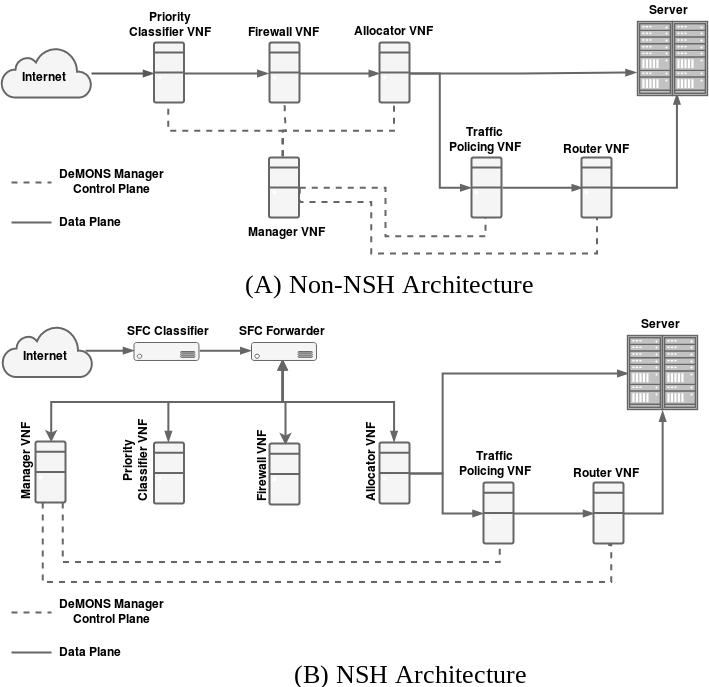
\includegraphics[width=.5\textwidth]{images/DeMONS.png}
\caption{DDoS Mitigation NFV Solution (DeMONS)}
\label{FIG:DeMONS}
\end{figure}


The DeMONS was deployed using the IETF's SFC architecture (\textit{i.e.}, Classifier and Service Function Forwarder) \cite{Joel-2015} and the VNF Platform prototype developed in this work. NSH was used to enable in-band control for sharing flow reputations and to orchestrate the traffic steering across all the employed NSH aware VNFs (\textit{i.e.}, the SFC). The reputation table (originally at the Manager) is now maintained by the Priority Classifier and shared between the VNFs through the NSH Context Header. In case of benign traffic, the Service Index is decremented by two in order to forward the packets directly to the Allocator, thus skipping the Firewall. Finally, the Allocator gets the reputation value directly from the flow packet by using the NSH's Context Header. Figure \ref{FIG:DeMONS}-B presents the adapted DeMONS implementation design.

% We deployed the DeMONS solution using the IETF's SFC architecture modules (\textit{i.e.}, Classifier and Service Function Forwarder) \cite{rfc7665} and the prototype VNF platform developed considering the architecture presented in Section \ref{ARCH}. We used the NSH to do in-band control of the flows reputations and coordination of the traffic steering across the DeMONS' SFC. We removed the shared reputation table from the Manager VNF and placed it locally at the Priority Classifier. The Priority Classifier uses that table and the IDS results to update the flow reputations, and, additionally, records the reputation value in the NSH's Context Header through the platform NSHP. Also, minor modifications were performed in the Priority Classifier NSHP's module in order to realized a double decremental in the Service Index for every flow with reputation greater than 0 during the NSH reinsertion. This Service Index manipulation skips the non-malicious traffic processing by the firewall, steering it directly to the Allocator. Finally, the Allocator gets the reputation value directly from the flow packet by using the NSHP's CH retrieve operation, without any VNF interaction. The Figure \ref{FIG:DeMONS}-B presents the adapted DeMONS implementation design.

The use of NSH led to performance improvements in DeMONS due to redesign and the embedded mechanism to exchange control data. The first experiment was executed to evaluate the execution time overhead introduced by retrieving and processing the reputations in both original and modified DeMONS. Two versions of the Packet Filter VNFC were developed in order to operate in both scenarios (NSH and Non-NSH), and were instrumented to measure the elapsed processing time for each packet. Iperf was used to generate the network traffic (UDP packets of 1470 Bytes), with the results presented in Figure \ref{FIG:DEMONSRRT}.

%Escala logaritimica
\begin{figure}[!htb]
\centering
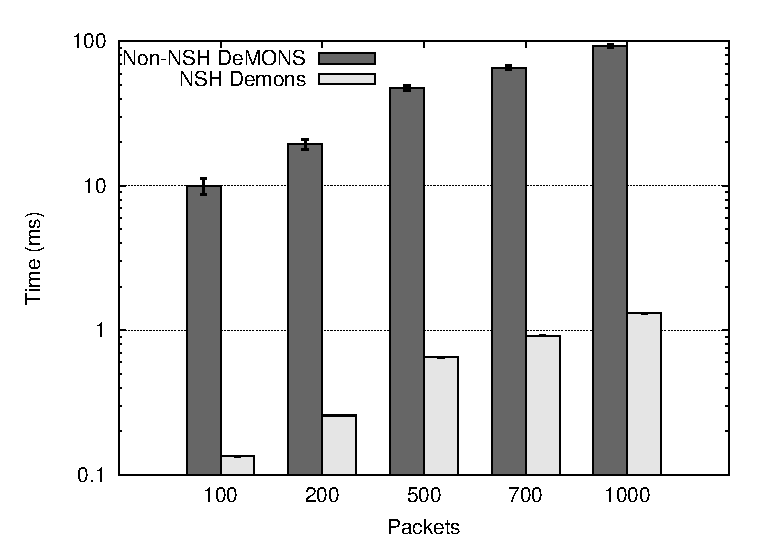
\includegraphics[width=.5\linewidth]{images/ExecTime.eps}
\caption{Reputation Retrieval Processing Time Overhead}
\label{FIG:DEMONSRRT}
\end{figure}

% \red{The use of NSH for the traffic steering and in-band control led to performance improvements in DeMONS. We analyzed the processing time overhead introduced by both the out band control (Non-NSH DeMONS) and in band control (NSH DeMONS) during the reputation retrieval for the DeMONS VNFs. To do that, an in band control VNFC and an out band control VNFC executing only the reputation retrieval operation were developed and deployed in the prototype platform. We instrumented the VNFCs in order to measure the execution time for every packet processed by them. Ours tests consists in traverse these VNFCs with 1470B UDP packets, created by the iperf tool, and aggregate the execution time for packets groups as exposed in Figure \ref{FIG:DEMONSRRT}.}

In the Non-NSH DeMONS, the reputation retrieval process consists in contacting the Manager (through a UDP Socket) to discover the reputations. This operation is performed for all the network packets traversing the VNFC. When NSH is employed, on the other hand, the reputation value is included in the NSH Context Header of each packet by the Priority Classifier. In this case, the Packet Filter just needs to open this header to retrieve the information. As suspected, the same operation (reputation retrieval) leads to significant differences in terms of processing time (in favor to NSH-based), which may affect other performance indicators (\textit{e.g.}, throughput and packet loss). An important observation is that no major differences occurred for packets with different sizes.
% \red{In the Non-NSH DeMONS, the reputation retrieval process consists on contacting the Manager (through an UDP Socket) to discover the reputations. This operation is performed for all the network packets traversing the VNFC. When NSH is employed, on the other hand, the reputation value is marked in the Context Header and its retrieving corresponds to just the local access of it. This operational difference leads to the Non-NSH DeMONS a reputation retrieval processing time overhead from 72 to 74 times greater than the NSH DeMONS. Once the extra processing time for this operation is imposed for each packet traversing the DeMONS VNFs, the RTT and throughput are directly affected according to the traffic volume growth. Also, it is important to notice that the package size do not change the reputation retrieval processing time (since the same operation is applied independently of this packet characteristic).}

The use of a Service Function Forwarder in the NSH DeMONS scenario also demonstrated interesting opportunities for improving the traffic steering overall. This SFC element (\textit{e.g.}, an OpenFlow Switch or a P4-enabled device) steers the network traffic according to the Service Index value present in the NSH Service Path Header. In this way, it is possible to manipulate the VNF execution order by updating the NSH Service Index according to decisions taken during VNF processing. For our case study, the Firewall VNF only processes the malicious traffic in order to collect statistics (\textit{e.g.}, number of discarded packets) and then discards the packets. In addition to not processing benign flows -- when malicious traffic is nonexistent (\textit{i.e.}, no attack occurring) -- it is possible to temporarily disable the Firewall VNF, thus saving computational resources.
% \red{Further, the traffic steering for the NSH DeMONS is more flexible than Non-NSH DeMONS due the use of a Service Function Forwarder. This SFC component steers the network traffic according to the Service Index present in the NSH Service Path Header. In this way, it is possible to manipulate the packet processing path by updating this NSH field according to decisions took during the VNFs processing. For our case study, the Firewall VNF only process the malicious traffic in order to collect statistics, such as the number of discarded packets, and finally drop it. In addition to not processing benign flows, when malicious traffic is inexistent (\textit{i.e.}, no attack occurring), its is possible to keep the Firewall VNF suspended, thus saving computational resources.}

%In Figure \ref{FIG:DEMONSFW}, for example, shows the aggregated processing time overhead measured internally for the Reputation Retrieval DeMONS VNFC (\textit{i.e.}, white box test), deployed in the prototype platform. Two different VNFCs were employed in this test: with out band control (Non-NSH DeMONS) and with in band control (NSH DeMONS). In the Non-NSH DeMONS, this processing consists on contacting the Manager (through an UDP Socket) to discover the reputations. This operation is performed for all the network packets traversing the network. When NSH is employed, on the other hand, the reputation value is marked in the Context Header and its retrieving corresponds to just the packet local access of it.

% and decide if the packet should be discarded (reputation equals to 0) or not.

% \blue{The application of NSH for the traffic steering and in band control makes possible to significantly improve the DeMONS NFs performance. For example, the Figure \ref{FIG:DEMONSFW} shows the aggregated packet processing time for the Firewall VNF with and without the use of NSH (developed using Python3 framework). The processing time measurement starts after the packet receiving by the NF, and stops before the packet sending operation. Thus, the Non-NSH DeMONS Firewall processing consists on the requisition of reputation value to the Manager (through a L3 UDP Socket) and the evaluation of that value in order to drop the packet (if it is 0) or forward it (other case). The NSH DeMONS Firewall, in turn, receives only the malicious traffic and a single operations is measured (\textit{i.e.}, the packet discarding). This operational difference between the Non-NSH DeMONS and NSH DeMONS Firewalls results in a large contrast in the processing time, being the first 72 to 77 times faster than the latter.}

%\red{In addition to the white box test, we analyzed the RTT overhead as a black box test for the same VNFCs also deployed in the prototype platform. To do that, we traversed the VNFs with an 1MBs UDP flow. The results seen in Figure \ref{FIG:DEMONSALLOC} show that the extra processing time introduced by the external reputation retrieval by the Non-NSH DeMONS is able to modify the average overall RTT when compared to the NSH DeMONS (difference of 0.2 milliseconds). Once the extra processing time for the reputation retrieval is imposed for every packet traversing the DeMONS VNFs, the RTT overhead may also grow for a higher traffic volume.}

%(also developed using Python3 framework) in order to measure the processing delay introduced by the reputation value retrieval

%\begin{figure}
%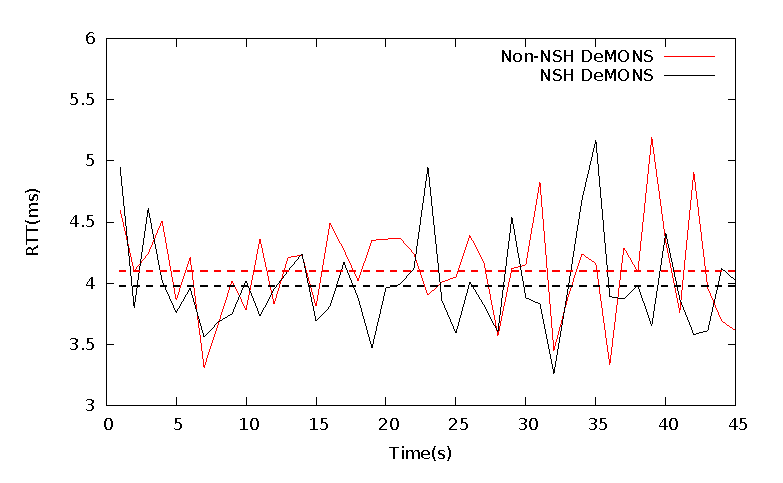
\includegraphics[width=\linewidth]{images/NSHAlloc.eps}
%\caption{Reputation Retrieval RTT}
%\label{FIG:DEMONSALLOC}
%\end{figure}

%%%%%
%\subsection{Heterogeneous Components Deployment}

%For the second case study, presented in Figure \ref{FIG:L7F}, the creation of a L7 Firewall employing the VNFC concept was evaluated. The ultimate goal of this network function is to block Skype traffic by using the fingerprint-based approach presented in \cite{Ehlert-2006}. The detection process consists on (i) port detection (80 and 443), (ii) payload pattern inspection (first 72 payload bytes), and (iii) the identification of similar data in different positions of the payload.

% In this case study we use the prototype platforms VNFCs support to deploy a complex function to realizing L7 filtering. We employed fingerprints presented in \cite{Ehlert-2006} to detect probable Skype traffic and block it. These fingerprints which are employed in this case study consists of port detection (80 and 443), payload pattern for port 443 (first 72 bytes), and payload segments self comparison for port 80.

%\begin{figure}[htb]
%\centering
%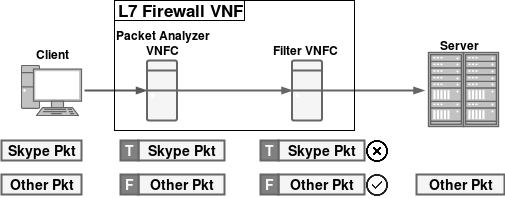
\includegraphics[width=.49\textwidth]{images/FirewallL7.png}
%\caption{L7 Firewall}
%\label{FIG:L7F}
%\end{figure}


%Two separate components were created: a packet analyzer and a packet filter. The packet analyzer was developed using the Python3 library Scapy\footnote{https://scapy.net/}, while the packet filter was implemented using both Python3 and CMR. The packet analyzer receives network traffic and verifies the destination port. All packets coming from ports 80/443 are marked and then forwarded, while the remaining packets are forwarded without marking. The marked packets received by the firewall are then processed in order to identify Skype fingerprints in the payload. If a Skype fingerprint is detected, the packet is marked as possible Skype. The second component (\textit{i.e.}, the packet filter) checks the marks and discards all the traffic that it considers to possibly be Skype traffic. These components were chained to create a L7 Firewall, although, they are independent and can be executed alone or be incorporated as part of other complex network functions.

% It is important to notice that the filter may block not only Skype traffic once, eventually, these Skype fingerprints can be employed by other applications.
% We developed a two components NF: Deep Packet Inspection (DPI) and a Firewall. The DPI was developed using Pyrhon3 language and Scapy library \footnote{https://scapy.net/}. This component receives the traffic and verifies the destination port. Every packet not addressed for port 80 or 443 is marked as non-Skype in the xxx byte of IP header and forwarded. The packets/frames addressed for port 80 and 443 are processed in order to identify the Skype fingerprints in the payload. After the payload analysis, if the processing returns true, the packet/frame is marked as possible Skype, else it is also marked as non-Skype. The second component (\textit{i.e.}, Firewall) checks the DPI marking and drops all the possible Skype traffic. It is important to notice that the Firewall may block not only SKype traffic once, eventually, these Skype fingerprints can be employed by other applications.

% We chained two components to create a sophisticated L7 Filter. These components, however, can be independently used or be incorporated as part of other complex functions. Also, we tested two firewalls implementations (\textit{i.e.}, Python3 and CMR) doing the same processing in order to identify performance differences between technologies combination. The case study is depicted in Figure \ref{FIG:L7F}.

%\begin{figure}[ht]
%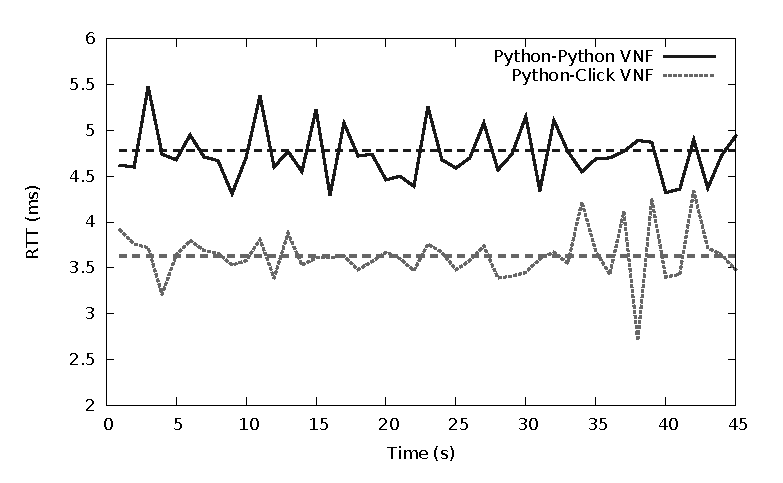
\includegraphics[width=\linewidth]{images/Delay.eps}
%\caption{L7 Firewall RTT}
%\label{FIG:L7FRTT}
%\end{figure}

% \vspace*{-1em}

%In this case study, we evaluated the RTT between the client and the server by using two combinations of VNFCS: both components were implemented in Python, and a mix of Python (for the Packet Analyzer) and CMR (for the Packet Filter). Figure \ref{FIG:L7FRTT} presents the results obtained from the experiments. It is possible to conclude that a combination of both programming languages is more appropriate to achieve better performance. It is important to notice, however, that although components implemented in CMR leverage its optimized packet processing, more sophisticated operations (\textit{e.g.}, analyzing the payload of ciphered packets) cannot be created using the default elements of this language. In these cases, Python 3 presents itself as an interesting approach to enable the development of advanced VNFCs with lower implementation efforts. Similar conclusions can be observed in other development scenarios, for example, when embedding assembly code in higher-level languages (\textit{e.g.}, C, C++), or when using the Java Native Interface (JNI) framework.
% \blue{Figure \ref{FIG:L7FRTT} presents the RTT measured during 45 seconds using Ping tool. Two VNFC combinations are employed in this test: the Python Packet Analyzer plus a Python Firewall, and the Python Packet Analyzer plus a CMR Firewall. The measured RTT varies from 4.4 to 5.5 milliseconds for python VNFCs combination, and from 2.9 to 4.4 for python and CMR combination. Once the same Python Packet Analyzer is used in both tests, the reduced RTT measurements verified by using a CMR Filter is attributed to its fastest modules, specially prepared for network traffic processing and previously compiled in a low-level programming language (C++). Despite presenting worse results in the RTT test, the Python3 programming framework still being an important piece to achieving higher flexibility and agility during the NFs development. Because of its general purpose, Python3 enables the implementation of sophisticated VNFCs (\textit{e.g.}, the presented Packet Analyzer) with lower efforts when compared to closed and monolithic frameworks, such as CMR.}

\section{Conclusion and Future Work}

Network Functions Virtualization (NFV) has been attracting great interest from both industry and academia. However, despite all the advancements in the field, there are still opportunities for research, development, and standardization. \blue{For example, there are no widely accepted definitions for the internal architecture of the platforms responsible for executing NFs, neither the processing of NSH inside those VNFs.} This leads to a scenario where several platforms (\textit{e.g.}, ClickOS and OpenNetVM) have been created without integration concerns in mind, the result is that none fulfills the complete set of NFV requirements.

% Virtualização de funções de rede tem atraído grande interesse de pesquisadores no mundo inteiro desde sua formalização inicial. Porém, apesar de chamar a atenção tanto da academia quanto da indústria, esse paradigma ainda não chegou a maturidade de conceitos, tecnologias e padronizações. Plataformas para execução de funções virtualizadas de rede se incluem nesse grupo onde, embora existam requisitos de alto nível para desenvolvimento das mesmas, há uma lacuna na literatura quanto sua organização arquitetural interna. Dessa forma, o desenvolvimento dessas plataforma é realizado sob demanda, resultando em soluções altamente heterogêneas e inflexíveis.

\blue{This work proposed a architecture for VNF Platforms with NSH support. We specified the basic modules for building a platform, as well as existing NFV enablers that can be employed. We also presented a platform prototype that employs the proposed architecture to support the execution of disparate network functions. Finally, we conducted a performance evalution on a case studies to identify the advantages of employing NSH on VNFs. We observed that creating VNFs with components implemented in different languages brings benefits regarding performance and development flexibility. The experiments show the advantages of using NSH when designing SFCs. First, the NSH Context-Header enables the functions to communicate and change information in-band. Second, the Service Index field allows the creation of dynamic SFCs, without the need to \textit{a priori} set the path of VNFs, also enabling traffic steering to be executed by using common solutions (e.g., Open vSwitch, P4-enabled equipment).}

% Este artigo apresenta uma proposta de arquitetura interna para plataformas destinadas a execução de funções de rede virtualizadas. Através do detalhamento dos blocos operacionais necessários em vista dos requisitos especificados, uma arquitetura genérica é discuta afim de dirigir os esforços de desenvolvimento a encontro de plataformas padronizadas, flexíveis e facilmente estendidas de acordo com o surgimento de novas tecnologias. Também, um protótipo de plataforma, intitulado Click-on-OSv, foi desenvolvido como prova de conceito, compreendendo, de maneira simplificada, os blocos operacionais previstos na arquitetura de referência apresentada. Finalmente, diversos aspectos operacionais da plataforma Click-on-OSv foram avaliados e comparados a outras soluções com objetivos semelhantes.

Future work includes the investigation on how the current VNF/SFC descriptors (\textit{e.g., TOSCA}) has to be adapted to support the concepts introduced in this work (\textit{i.e.,} NSH and VNFCs). Furthermore, it is our plan to continue working and improve the prototype by supporting novel packet processing frameworks (\textit{e.g.,} VPP) and other virtual network technologies (\textit{e.g.,} netmap).

%\section*{Acknowledgements}

%This research was performed partially within the project GT-FENDE. The authors would like to thank Rede Nacional de Ensino e Pesquisa (RNP), for their support to the GT-FENDE project.


% As future work, we aim to improve the architecture presented in this paper by detailing the components Dispatcher and NSH Processor, and discussing how the current VNF/SFC descriptors must be adapted to support novel VNF platforms. Finally, improvements in the Click-on-OSv will be conducted to support other virtual network technologies and packet processing frameworks, as well as to improve its performance.

% Em trabalhos futuros objetiva-se aprofundar as especificações arquiteturais de plataformas para execução de funções virtualizadas de rede através do desenvolvimento de um documento de especificação ricamente detalhado. Através desse busca-se solidificar os requisitos mínimos e modelos de desenvolvimento para cada bloco operacional interno, além de apontar modificações necessárias nos descritores de funções e serviços existentes para suportarem tal arquitetura. Ainda, uma análise profunda de diferentes tipos de NFV \textit{Enablers} será realizada com o objetivo de observar não só o desempenho de processamento de pacotes, mas também o impacto da ativação, desativação e/ou substituição dos mesmos em diferentes cenários de uso. Finalmente, aprimoramentos no protótipo de plataforma Click-on-OSv serão realizados com o intuíto de disponibilizar diferentes ferramentas para a rede virtual e \textit{frameworks} para o processamento de pacotes, concretizando este como uma opção completa, genérica e flexível para execução de VNFs.


\bibliographystyle{spbasic}
\bibliography{bibliografia.bib}

\end{document}
